+++Motivate motivate motivate+++\\
Nonlinear evolution equations ubiquitous across the sciences. These typically take the form
$$ \dot{x}(t) = F\left(x(t)\right)$$ where $x\in \mathbf{R}^d, F\in C^r(\mathbf{R}^d,\mathbf{R}^d)$. We will be interested in systems that occur on different timescales, known as fast-slow systems. These occur naturally in physics, neuroscience and many other biological scenarios +++ Van der Pol, FitzHugh-Nagumo, other bio ref?+++. Models of such systems can be written generally in the form given below.
\begin{align}
\begin{cases}
x' &=\frac{dx}{dt}= f(x,y,\epsilon),\\
y' &= \frac{dy}{dt}= \epsilon g(x,y,  \epsilon),
\end{cases}\label{FastS}
\end{align} 
Here, $x \in \R^n, y \in \R^m, m,n \geq 1$ and $f,g$ are sufficiently smooth. The separation in timescales is governed by $0<\epsilon \ll 1$, known as the timescale separation parameter. Some systems also act on more than two timescales, in which case there is more than one timescale separation parameter.  In the system above, note that the change in $x$ is $O(1)$, whilst it is $O(\epsilon)$ in $y$. As $\epsilon$ is very small, this means that the change in $x$ is much faster than that of $y$. If we slow down time with the transformation $\tau = \epsilon t$, the system becomes  
\begin{align}
	\begin{cases}
	\epsilon \dot{x} &= \epsilon \frac{dx}{d\tau} = f(x,y,\lambda, \epsilon),\\
	\dot{y} & = \frac{dy}{d \tau} =  g( x,y, \lambda, \epsilon),
	\end{cases}\label{SlowS}
\end{align} 
Represented like this, $\dot{x} = O(\frac{1}{\epsilon})$ whilst $\dot{y} = O(1)$.  The time scale given by $\tau$ is said to be slow so (\ref{SlowS}) is the \emph{slow system} while (\ref{FastS}) is the \emph{fast system}.\\


\begin{figure}[h]
	%\includegraphics[]}
	\caption{Examples of fast-slow systems in nature (neuron,ECG etc. )}
	\label{fig:nature}
\end{figure} 


Throughout what follows, the motivating example will be the Van der Pol equation. The Van der Pol oscillator is a well-studied second order ODE that is used to model a variety of physical and biological phenomena. It was developed by the Dutch physicist and electrical engineer Balthasar Van der Pol, who conducted research on electrical circuits. It describes the evolution of the position coordinate \(x(t)\) according to the following the ODE:
\begin{equation} \label{eq:vdP}
\ddot{x}(t)-\mu\left(1-x^2(t)\right)\dot{x}(t)+x(t)=0,
\end{equation}
where \(\mu \gg 1\) is a scalar constant. This equation can be scaled so that it becomes a two dimensional fast-slow system of the form shown in Equation (\ref{FastS}) after a change of variables.

\begin{equation}
\begin{aligned}
&x'=-y+x^2-\frac{x^3}{3} \\
&y'=\epsilon(-\lambda+x)
\end{aligned}
\label{eq: canonical}
\end{equation}

When presented with any dynamical system, the aim is to fully understand the global dynamics of the system. A numerical simulation is often a good first step. Setting $\lambda=\epsilon=1$ gives the phase plane given in Figure \ref{fig:VDPE1}.
\begin{figure}[]
	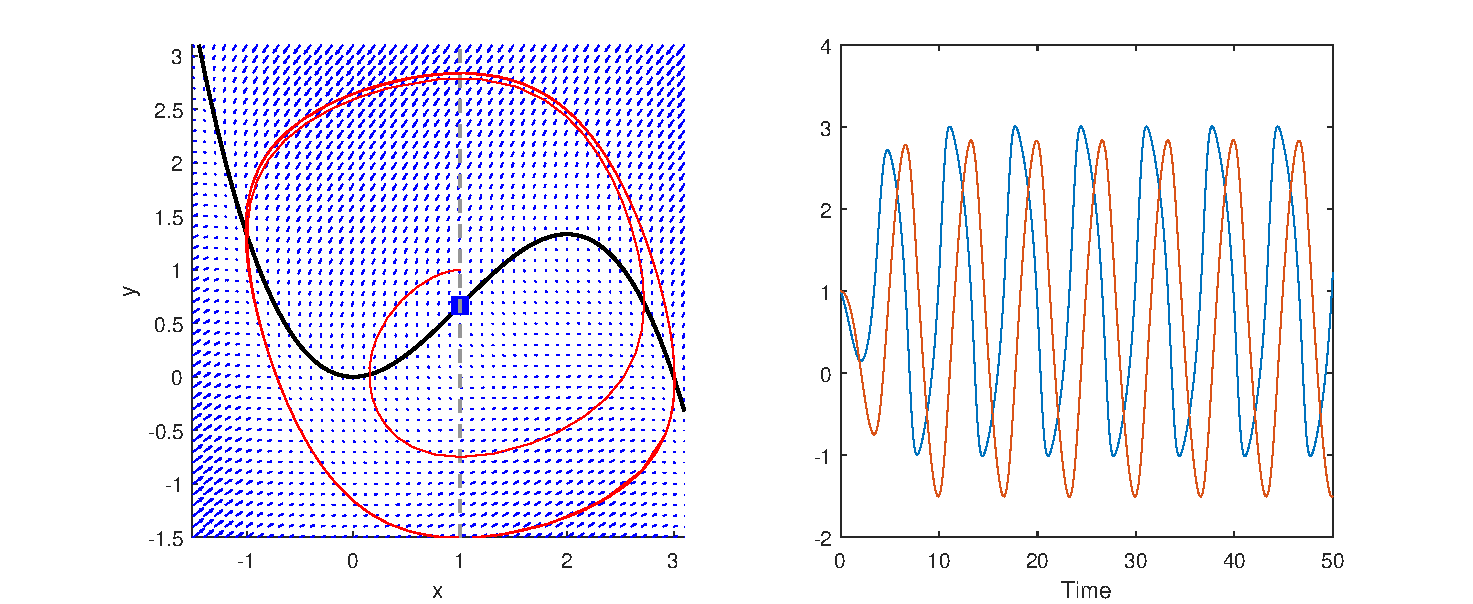
\includegraphics[width=\textwidth]{VDPbigE}
	\caption[Van der Pol Dynamics with \texorpdfstring{$\epsilon=1$}{eps=1}]{Phase plane and time series of the \vdp for $\epsilon=\lambda=1$ started from $(1,1)$. The dashed line indicates the null cline in $y$ while that in $x$ is given by the solid black line. The equilibrium is highlighted in blue.}
	\label{fig:VDPE1}
\end{figure}
Figure \ref{fig:VDPE1} shows the presence of a  periodic large amplitude oscillation, which Van der Pol called \emph{relaxation oscillations}. Setting $\epsilon=1$ means that there is no separation in timescale. Figure \ref{fig:VDPE01} shows a more realistic scenario, when $\epsilon=0.01$. Here there is what appears to be an almost instantaneous change in $x$ every 800 time steps. What causes this rapid change? We wish to find a rigorous reason for this jump from slow to fast movement. A natural starting point would be to study what happens when $\epsilon=0$, that is, when this rapid change is in fact instantaneous. Doing so in both the fast and slow system will give two different views of the dynamics.
\begin{figure}[]
	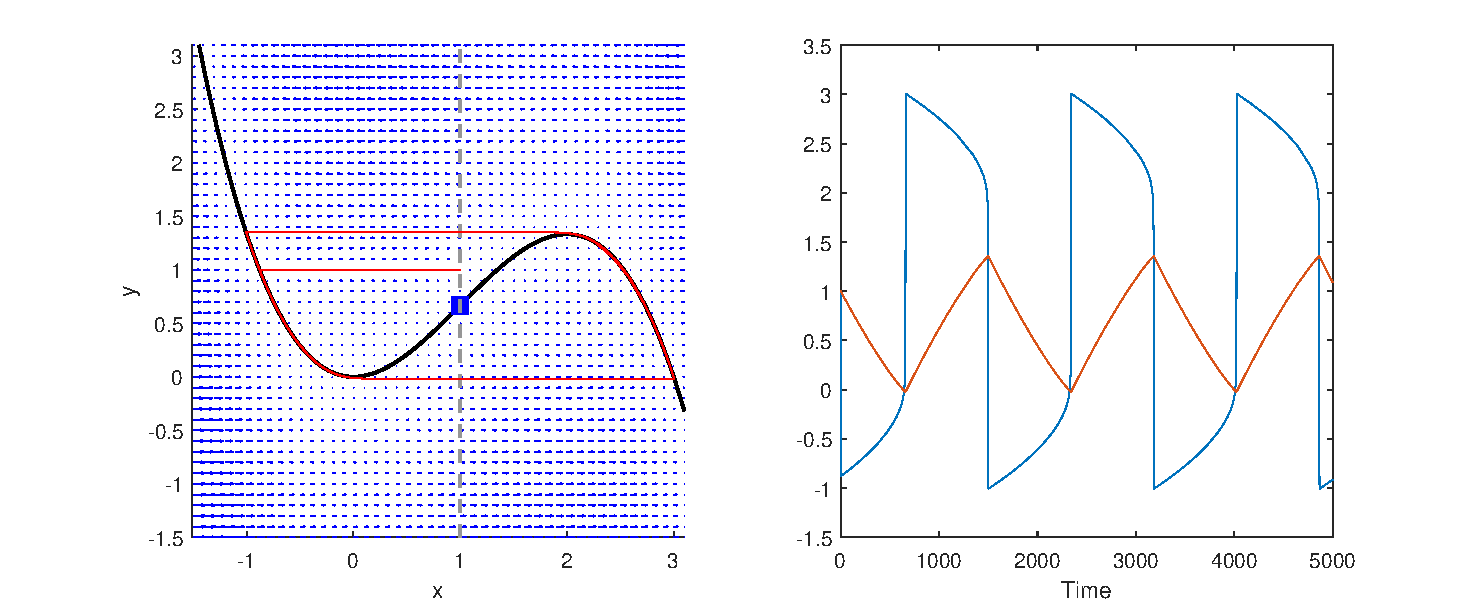
\includegraphics[width=\textwidth]{VDPsmallE}
	\caption[Van der Pol Dynamics with \texorpdfstring{$\epsilon=0.01$}{eps=0.1}]{Phase plane and time series of the \vdp for $\epsilon=0.01, \lambda=1$ started from $(1,1)$. The dashed line indicates the null cline in $y$ while that in $x$ is given by the solid black line. The equilibrium is highlighted in blue.}
	\label{fig:VDPE01}
\end{figure}
 Taking the limit $\epsilon \to 0$ in the fast system (\ref{FastS}) gives, \begin{align} \label{FastS0}
		\begin{cases}
			x' &=\frac{dx}{dt}= f(x,y,\lambda, \epsilon)\\
			y' &= 0.
		\end{cases}
	\end{align}
This is known as the \emph{layer problem} as movement is restricted to the layers $y=const.$ and similarly taking the limit in the slow system (\ref{SlowS}) gives
	\begin{align}\label{SlowS0}
		\begin{cases}
			0 &= \epsilon \frac{dx}{d \tau} = f(x,y,\lambda, 0)\\
			\dot{y} & = \frac{dy}{d \tau} =  g( x,y, \lambda,0).
		\end{cases}
	\end{align}
This is known as the \emph{reduced problem} as the dynamics are reduced from the whole plane to the line $f=0$. The set $S= \{ (x,y) : f(x,y,0)=0 \} = \left\{ (x,y) : y = x^2-\dfrac{x^3}{3}\right \}$ is called the \emph{critical manifold}. We thus have two separate systems that combine to illustrate the global dynamics when $\epsilon =0$ and $\lambda = 1$. It remains to show that the flow in these limiting cases persists under perturbation to $0<\epsilon \ll 1$ and ascertain whether the behaviour is the same for all $\lambda$. We shall restrict our attention to the jump at $(0,0)$, the case for the point $(2,\frac{4}{3}$ is analogous. The aim is to fully understand the dynamics in a neighbourhood of these jump points for $\epsilon \ll 1$.

\subsection{Reduced Dynamics}
In order to determine the reduced dynamics on the critical manifold $S$, we consider the reduced problem (\ref{SlowS0}). The critical manifold is  an S-shaped curve. Since the flow on $S$ is determined by $\dot{y}$, it can be seen that since the sign of $g$ is negative in the neighbourhood of the point $(0,0)$, the slow flow on $S$ is directed towards this point.

The two  fold points $(x_0^\pm,y_0^\pm)$ coincide with the extrema of the cubic function  $ \phi(x) = y = x^2-\dfrac{x^3}{3}$.
Then using the chain rule, the second Equation of \ref{eq: reduced g} is  \citep{krupa2001},
\begin{equation}
\phi_x(x)\dot{x}=g(x,\phi(x),0).
\label{eq: general reduced}
\end{equation}
Rearranging this gives an expression for the dynamics in $x$ on $S$.
We find that $\phi(x)=x^2-\dfrac{x^3}{3}$, where the derivative \wrt $x$ gives $\phi_x(x)=2x-x^2$.
Therefore Equation \ref{eq: general reduced} becomes 
\begin{align*}
\dot{x} = \frac{g(x,\phi(x),0)}{ \phi_x(x)} = \frac{ x-1}{2x-x^2} =\frac{ x-1}{x(2-x)}.
\end{align*}
This calculation confirms that the fold points at $x=0$ and $x=2$ are singularities of the reduced system. Therefore, no conclusions about the dynamics of $x$ can be made at the fold points. 


Section \ref{GSPT} gives conditions under which the dynamics persist for small $\epsilon$. Section \ref{sec:singularitiesandfoldpoints} addresses the shortcomings of the previous theory and motivates the introduction of the blow up method which is applied in Section \ref{sec: VDP Blowup}. The case when $\lambda \neq 1$ is considered in Section \ref{sec:canard-points}. Section \ref{sec: threedimfolds} then begins to look at higher dimensional fast-slow systems.




Now considering Equation \ref{SlowS0}, we can write $f(x,y,\lambda, 0)=0$. Then we are able to define the critical manifold as:,
	\begin{align} \label{CriticalS}
		S= \left\{ (x,y) : f(x,y,\lambda, 0)=0 \right \},
	\end{align}
where, by definition of $S$, the points $(x,y) \in S$ are equilibria of (\ref{FastS0}). Before we continue, it is useful to have a visual interpretation of these flows,
\begin{figure}[h!]\centering
	\begin{subfigure}[t]{0.45\textwidth}
		\centering
		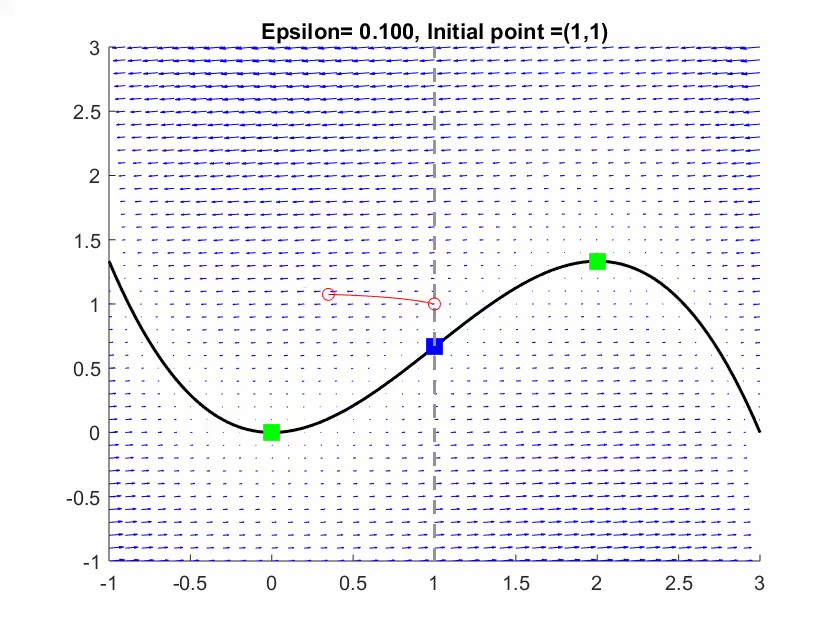
\includegraphics[width=.8\linewidth]{vdPhopf-Moment-1.jpg}
		\caption{The initial flow within the system starting at $ (x,y)=(1,1) $.}
	\end{subfigure}
	\hfill
	\begin{subfigure}[t]{0.45\textwidth}
		\centering
		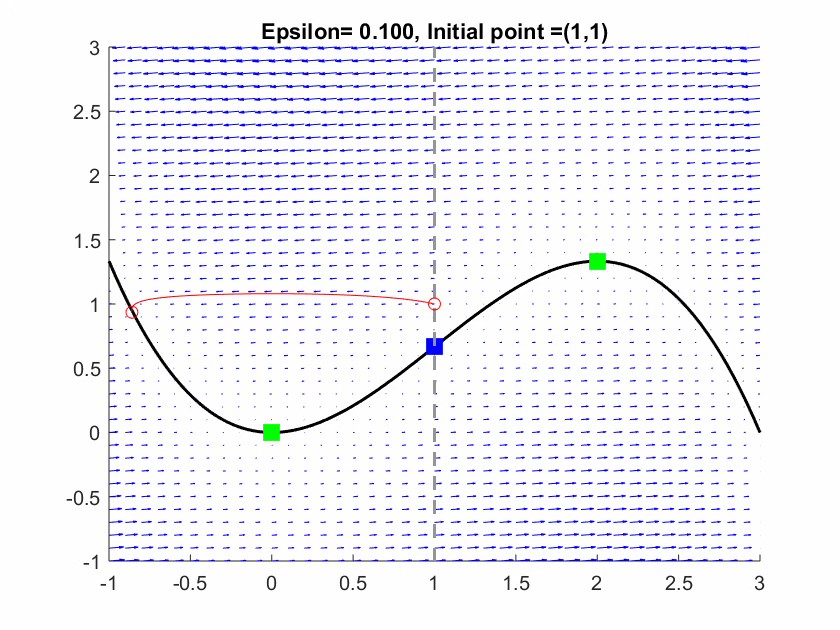
\includegraphics[width=.8\linewidth]{vdPhopf-Moment-2.jpg}
		\caption{The flow as it hits the slow manifold.}
	\end{subfigure}

	\vspace{1cm}
	\begin{subfigure}[t]{0.45\textwidth}
		\centering
		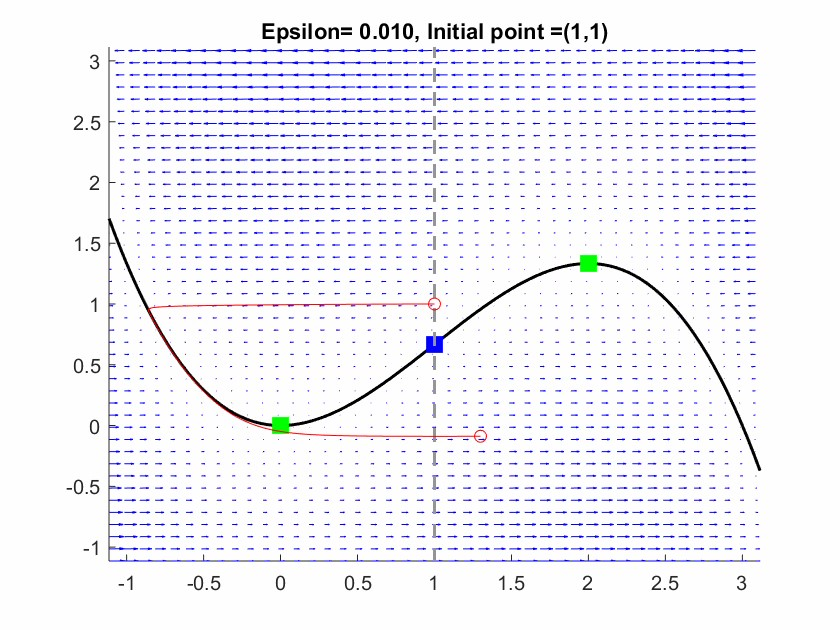
\includegraphics[width=.8\linewidth]{vdp-jump1}
		\caption{The flow as it intersects with the fold point and begins the jump.}
	\end{subfigure}
	\hfill
	\begin{subfigure}[t]{0.45\textwidth}\centering
		% just an empty subfigure to shift C below A
		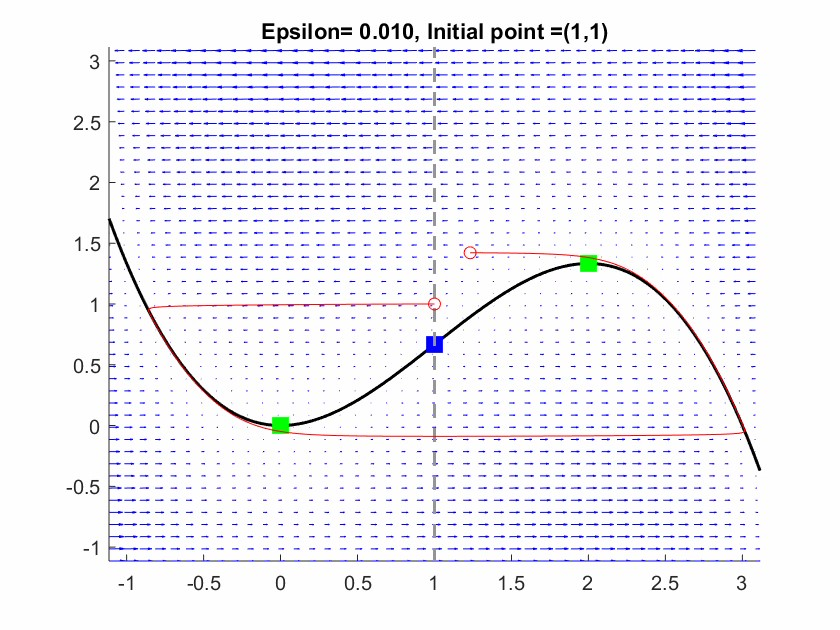
\includegraphics[width=.8\linewidth]{vdp-jump2}
		\caption{The second jump before continuing in a periodic fashion.}
	\end{subfigure}
	\caption{Flows in the \vdp system.}
	\label{fig: vdp flow diagram}
\end{figure}



